% $Id: examples.Rnw 66 2010-09-03 08:50:26Z jranke $
%%\VignetteIndexEntry{Examples for kinetic evaluations using mkin}
%%VignetteDepends{FME}
%%\usepackage{Sweave}
\documentclass[12pt,a4paper]{article}
\usepackage{a4wide}
%%\usepackage[lists,heads]{endfloat}
\usepackage{booktabs}
\usepackage{amsfonts}
\usepackage{latexsym}
\usepackage{amsmath}
\usepackage{amssymb}
\usepackage{graphicx}
\usepackage{parskip}
\usepackage[round]{natbib}
\usepackage{amstext}
\usepackage{hyperref}
\usepackage[utf8]{inputenc}

\newcommand{\Rpackage}[1]{{\normalfont\fontseries{b}\selectfont #1}}
\newcommand{\Robject}[1]{\texttt{#1}}
\newcommand{\Rclass}[1]{\textit{#1}}
\newcommand{\Rcmd}[1]{\texttt{#1}}

\newcommand{\RR}{\textsf{R}}

\RequirePackage[T1]{fontenc}
\RequirePackage{graphicx,ae,fancyvrb}
\IfFileExists{upquote.sty}{\RequirePackage{upquote}}{}
\usepackage{relsize}

\DefineVerbatimEnvironment{Sinput}{Verbatim}{baselinestretch=1.05}
\DefineVerbatimEnvironment{Soutput}{Verbatim}{fontfamily=courier,
                                              baselinestretch=1.05,
                                              fontshape=it,
                                              fontsize=\relsize{-1}}
\DefineVerbatimEnvironment{Scode}{Verbatim}{}  
\newenvironment{Schunk}{}{}

\hypersetup{  
  pdftitle = {Examples for kinetic evaluations using mkin},
  pdfsubject = {Manuscript},
  pdfauthor = {Johannes Ranke},
  colorlinks = {true},
  linkcolor = {blue},
  citecolor = {blue},
  urlcolor = {red},
  hyperindex = {true},
  linktocpage = {true},
}

\begin{document}
\title{Examples for kinetic evaluations using mkin}
\author{\textbf{Johannes Ranke} \\[0.5cm]
%EndAName
Eurofins Regulatory AG\\
Weidenweg 15, CH--4310 Rheinfelden, Switzerland\\[0.5cm]
and\\[0.5cm]
University of Bremen\\
}
\maketitle

%\begin{abstract}
%\end{abstract}


\thispagestyle{empty} \setcounter{page}{0}

\clearpage

\tableofcontents

\textbf{Key words}: Kinetics, FOCUS, nonlinear optimisation

\section{Kinetic evaluations for parent compounds}
\label{intro}

These examples are also evaluated in a parallel vignette of the
\Rpackage{kinfit} package \citep{pkg:kinfit}. The datasets are from Appendix 3,
of the FOCUS kinetics report \citep{FOCUS2006, FOCUSkinetics2011}.

\subsection{Laboratory Data L1}

The following code defines example dataset L1 from the FOCUS kinetics
report, p. 284

\begin{Schunk}
\begin{Sinput}
R> library("mkin")
R> FOCUS_2006_L1 = data.frame(
+   t = rep(c(0, 1, 2, 3, 5, 7, 14, 21, 30), each = 2),
+   parent = c(88.3, 91.4, 85.6, 84.5, 78.9, 77.6, 
+              72.0, 71.9, 50.3, 59.4, 47.0, 45.1,
+              27.7, 27.3, 10.0, 10.4, 2.9, 4.0))
R> FOCUS_2006_L1_mkin <- mkin_wide_to_long(FOCUS_2006_L1)
\end{Sinput}
\end{Schunk}

The next step is to set up the models used for the kinetic analysis. Note that
the model definitions contain the names of the observed variables in the data.
In this case, there is only one variable called \Robject{parent}.

\begin{Schunk}
\begin{Sinput}
R> SFO <- mkinmod(parent = list(type = "SFO"))
R> FOMC <- mkinmod(parent = list(type = "FOMC"))
R> DFOP <- mkinmod(parent = list(type = "DFOP"))
\end{Sinput}
\end{Schunk}

The three models cover the first assumption of simple first order (SFO),
the case of declining rate constant over time (FOMC) and the case of two
different phases of the kinetics (DFOP). For a more detailed discussion
of the models, please see the FOCUS kinetics report.

The following two lines fit the model and produce the summary report
of the model fit. This covers the numerical analysis given in the 
FOCUS report.

\begin{Schunk}
\begin{Sinput}
R> m.L1.SFO <- mkinfit(SFO, FOCUS_2006_L1_mkin, quiet=TRUE)
R> summary(m.L1.SFO)
\end{Sinput}
\begin{Soutput}
mkin version:    0.9.10 
R version:       2.15.2 
Date of fit:     Sat Feb 16 21:38:15 2013 
Date of summary: Sat Feb 16 21:38:15 2013 

Equations:
[1] d_parent = - k_parent_sink * parent

Starting values for optimised parameters:
              initial   type transformed
parent_0        100.0  state  100.000000
k_parent_sink     0.1 deparm   -2.302585

Fixed parameter values:
None

Optimised, transformed parameters:
              Estimate Std. Error
parent_0        92.471      1.368
k_parent_sink   -2.347      0.041

Backtransformed parameters:
              Estimate
parent_0        92.471
k_parent_sink    0.096

Residual standard error: 2.948 on 16 degrees of freedom

Chi2 error levels in percent:
         err.min n.optim df
All data   3.424       2  7
parent     3.424       2  7

Estimated disappearance times:
        DT50  DT90
parent 7.249 24.08

Estimated formation fractions:
            ff
parent_sink  1

Parameter correlation:
              parent_0 k_parent_sink
parent_0        1.0000        0.6248
k_parent_sink   0.6248        1.0000

Data:
 time variable observed predicted residual
    0   parent     88.3    92.471  -4.1710
    0   parent     91.4    92.471  -1.0710
    1   parent     85.6    84.039   1.5610
    1   parent     84.5    84.039   0.4610
    2   parent     78.9    76.376   2.5241
    2   parent     77.6    76.376   1.2241
    3   parent     72.0    69.412   2.5884
    3   parent     71.9    69.412   2.4884
    5   parent     50.3    57.330  -7.0301
    5   parent     59.4    57.330   2.0699
    7   parent     47.0    47.352  -0.3515
    7   parent     45.1    47.352  -2.2515
   14   parent     27.7    24.247   3.4527
   14   parent     27.3    24.247   3.0527
   21   parent     10.0    12.416  -2.4163
   21   parent     10.4    12.416  -2.0163
   30   parent      2.9     5.251  -2.3513
   30   parent      4.0     5.251  -1.2513
\end{Soutput}
\end{Schunk}

A plot of the fit is obtained with the plot function for mkinfit objects.

\begin{Schunk}
\begin{Sinput}
R> plot(m.L1.SFO)
\end{Sinput}
\end{Schunk}
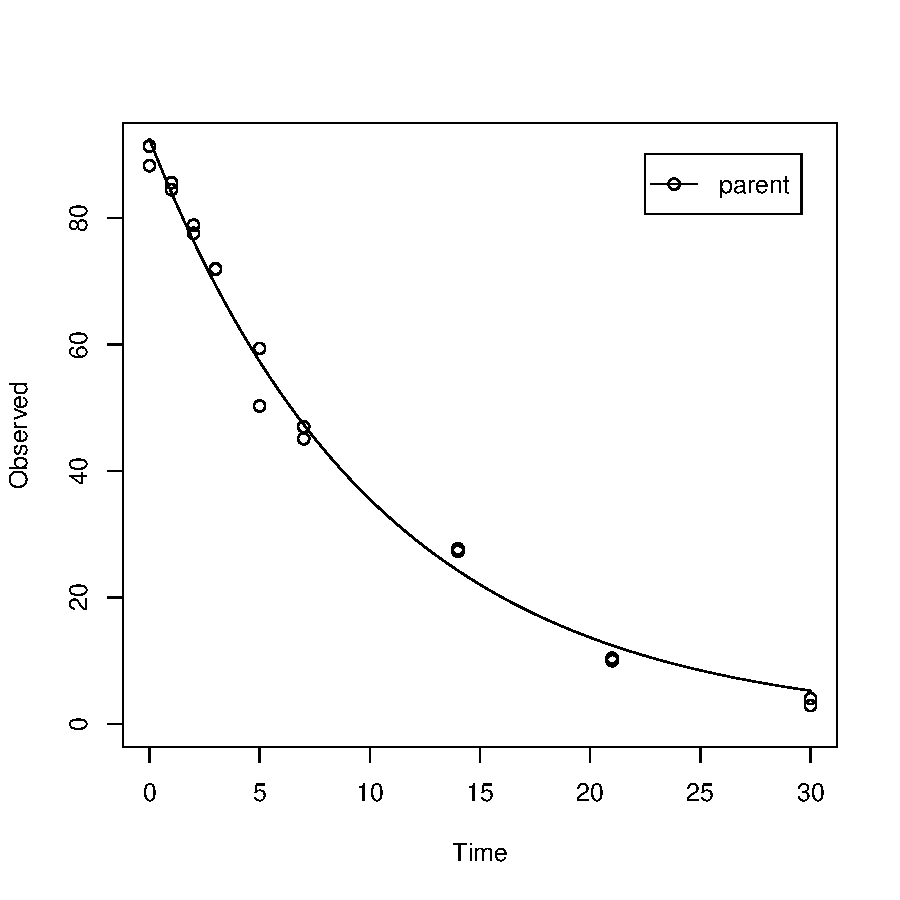
\includegraphics{examples-L1_SFO_plot}

The residual plot can be obtained using the information contained in the
mkinfit object, which is in fact a derivative of an modFit object defined by
the \Rpackage{FME} package.

\begin{Schunk}
\begin{Sinput}
R> plot(m.L1.SFO$data$time, m.L1.SFO$data$residual,
+   xlab = "Time", ylab = "Residual", ylim = c(-8, 8))
R> abline(h = 0, lty = 2)
\end{Sinput}
\end{Schunk}
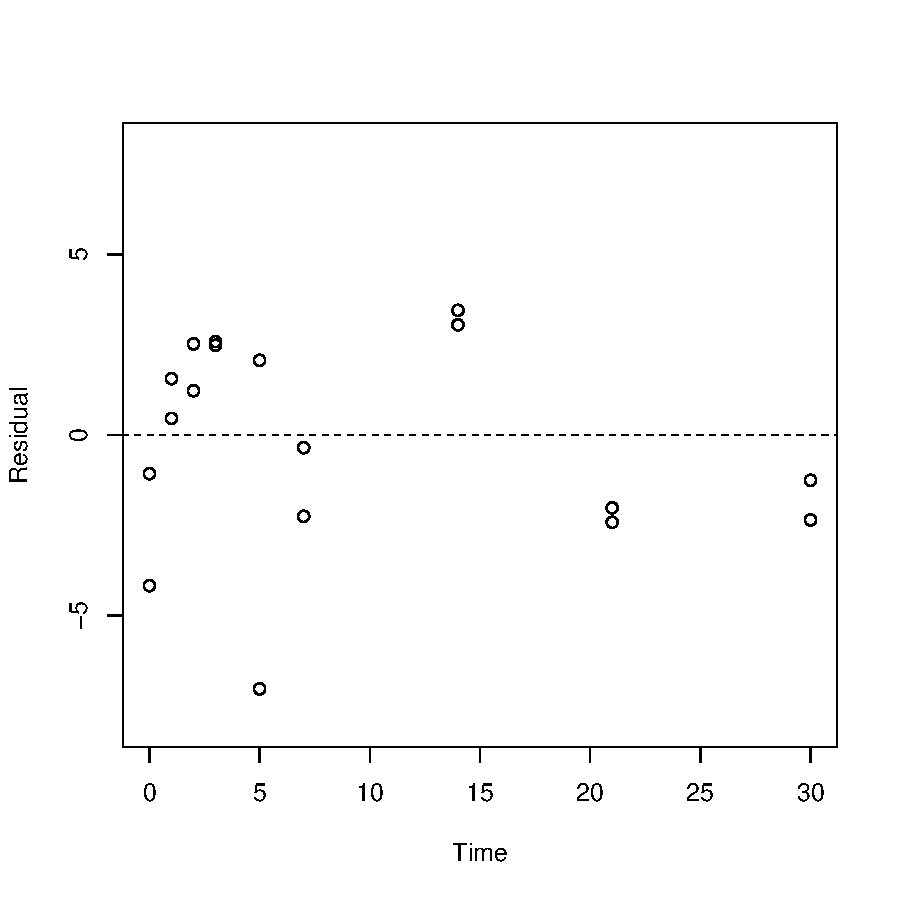
\includegraphics{examples-L1_SFO_residuals}

For comparison, the FOMC model is fitted as well, and the $\chi^2$ error level
is checked.

\begin{Schunk}
\begin{Sinput}
R> m.L1.FOMC <- mkinfit(FOMC, FOCUS_2006_L1_mkin, quiet=TRUE)
R> s.m.L1.FOMC <- summary(m.L1.FOMC)
R> s.m.L1.FOMC$errmin
\end{Sinput}
\begin{Soutput}
            err.min n.optim df
All data 0.03618911       3  6
parent   0.03618911       3  6
\end{Soutput}
\end{Schunk}

Due to the higher number of parameters, and the lower number of degrees of freedom
of the fit, the $\chi^2$ error level is actually higher for the FOMC model (3.6\%) than 
for the SFO model (3.4\%).

\subsection{Laboratory Data L2}

The following code defines example dataset L2 from the FOCUS kinetics
report, p. 287

\begin{Schunk}
\begin{Sinput}
R> library("mkin")
R> FOCUS_2006_L2 = data.frame(
+   t = rep(c(0, 1, 3, 7, 14, 28), each = 2),
+   parent = c(96.1, 91.8, 41.4, 38.7,
+              19.3, 22.3, 4.6, 4.6,
+              2.6, 1.2, 0.3, 0.6))
R> FOCUS_2006_L2_mkin <- mkin_wide_to_long(FOCUS_2006_L2)
\end{Sinput}
\end{Schunk}

Again, the SFO model is fitted and a summary is obtained.

\begin{Schunk}
\begin{Sinput}
R> m.L2.SFO <- mkinfit(SFO, FOCUS_2006_L2_mkin, quiet=TRUE)
R> summary(m.L2.SFO)
\end{Sinput}
\begin{Soutput}
mkin version:    0.9.10 
R version:       2.15.2 
Date of fit:     Sat Feb 16 21:38:15 2013 
Date of summary: Sat Feb 16 21:38:15 2013 

Equations:
[1] d_parent = - k_parent_sink * parent

Starting values for optimised parameters:
              initial   type transformed
parent_0        100.0  state  100.000000
k_parent_sink     0.1 deparm   -2.302585

Fixed parameter values:
None

Optimised, transformed parameters:
              Estimate Std. Error
parent_0       91.4656      3.807
k_parent_sink  -0.4112      0.107

Backtransformed parameters:
              Estimate
parent_0        91.466
k_parent_sink    0.663

Residual standard error: 5.51 on 10 degrees of freedom

Chi2 error levels in percent:
         err.min n.optim df
All data   14.38       2  4
parent     14.38       2  4

Estimated disappearance times:
        DT50  DT90
parent 1.046 3.474

Estimated formation fractions:
            ff
parent_sink  1

Parameter correlation:
              parent_0 k_parent_sink
parent_0        1.0000        0.4295
k_parent_sink   0.4295        1.0000

Data:
 time variable observed     predicted residual
    0   parent     96.1 91.4656079103   4.6344
    0   parent     91.8 91.4656079103   0.3344
    1   parent     41.4 47.1395280371  -5.7395
    1   parent     38.7 47.1395280371  -8.4395
    3   parent     19.3 12.5210295280   6.7790
    3   parent     22.3 12.5210295280   9.7790
    7   parent      4.6  0.8833842647   3.7166
    7   parent      4.6  0.8833842647   3.7166
   14   parent      2.6  0.0085318162   2.5915
   14   parent      1.2  0.0085318162   1.1915
   28   parent      0.3  0.0000007958   0.3000
   28   parent      0.6  0.0000007958   0.6000
\end{Soutput}
\end{Schunk}

The $\chi^2$ error level of 14\% suggests that the model does not fit very well.
This is also obvious from the plots of the fit and the residuals.

\begin{Schunk}
\begin{Sinput}
R> plot(m.L2.SFO)
\end{Sinput}
\end{Schunk}
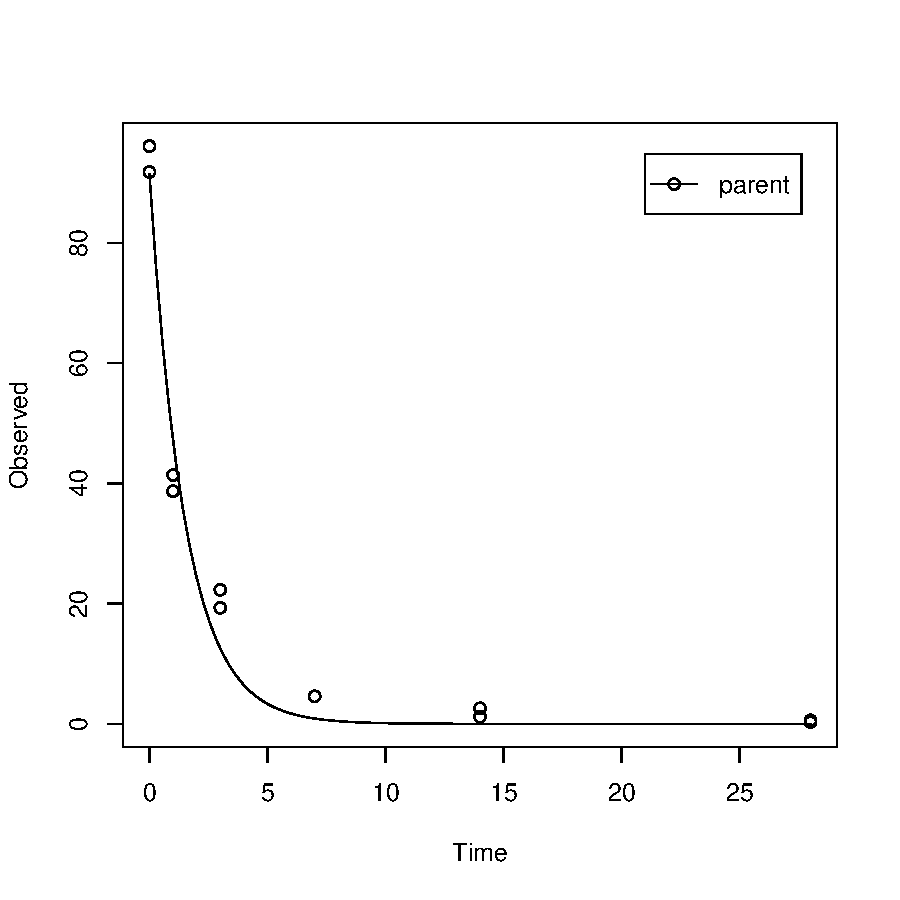
\includegraphics{examples-L2_SFO_plot}

In the FOCUS kinetics report, it is stated that there is no apparent systematic
error observed from the residual plot up to the measured DT90 (approximately at
day 5), and there is an underestimation beyond that point.

\begin{Schunk}
\begin{Sinput}
R> plot(m.L2.SFO$data$time, m.L2.SFO$data$residual,
+   xlab = "Time", ylab = "Residual", ylim = c(-10, 10))
R> abline(h = 0, lty = 2)
\end{Sinput}
\end{Schunk}
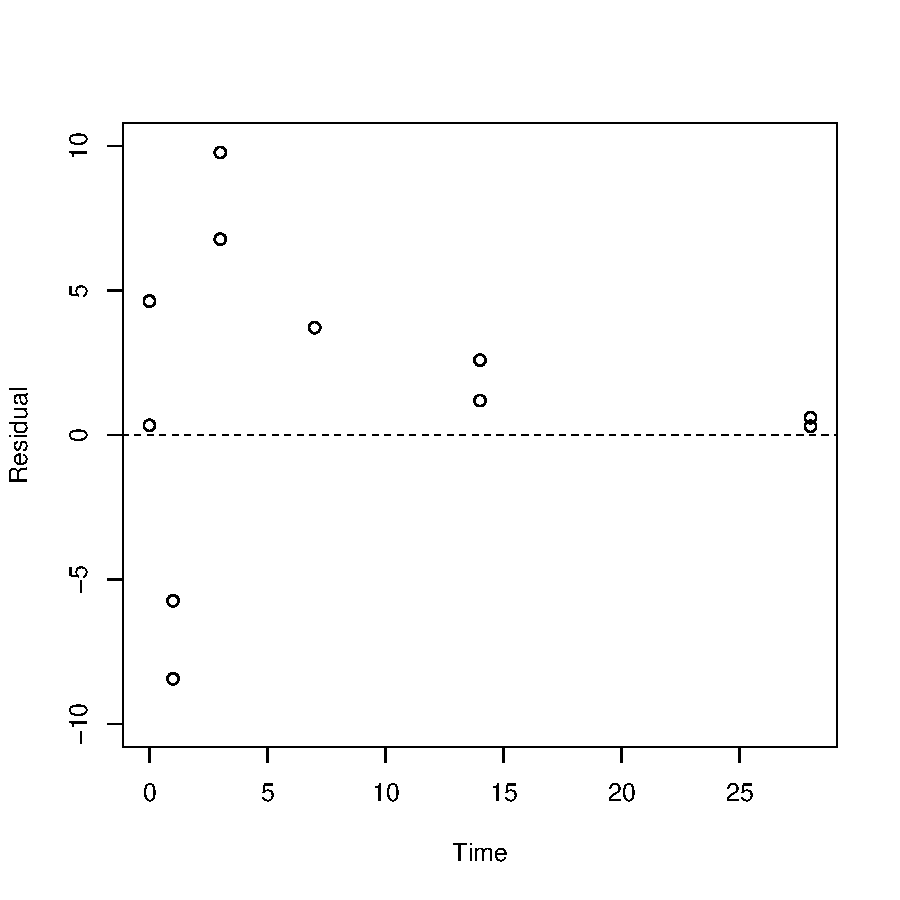
\includegraphics{examples-L2_SFO_residuals}

We may add that it is difficult to judge the random nature of the residuals just 
from the three samplings at days 0, 1 and 3. Also, it is not clear why a
consistent underestimation after the approximate DT90 should be irrelevant.

For comparison, the FOMC model is fitted as well, and the $\chi^2$ error level
is checked.

\begin{Schunk}
\begin{Sinput}
R> m.L2.FOMC <- mkinfit(FOMC, FOCUS_2006_L2_mkin, quiet=TRUE)
R> plot(m.L2.FOMC)
R> s.m.L2.FOMC <- summary(m.L2.FOMC)
R> s.m.L2.FOMC$errmin
\end{Sinput}
\begin{Soutput}
            err.min n.optim df
All data 0.06204245       3  3
parent   0.06204245       3  3
\end{Soutput}
\end{Schunk}
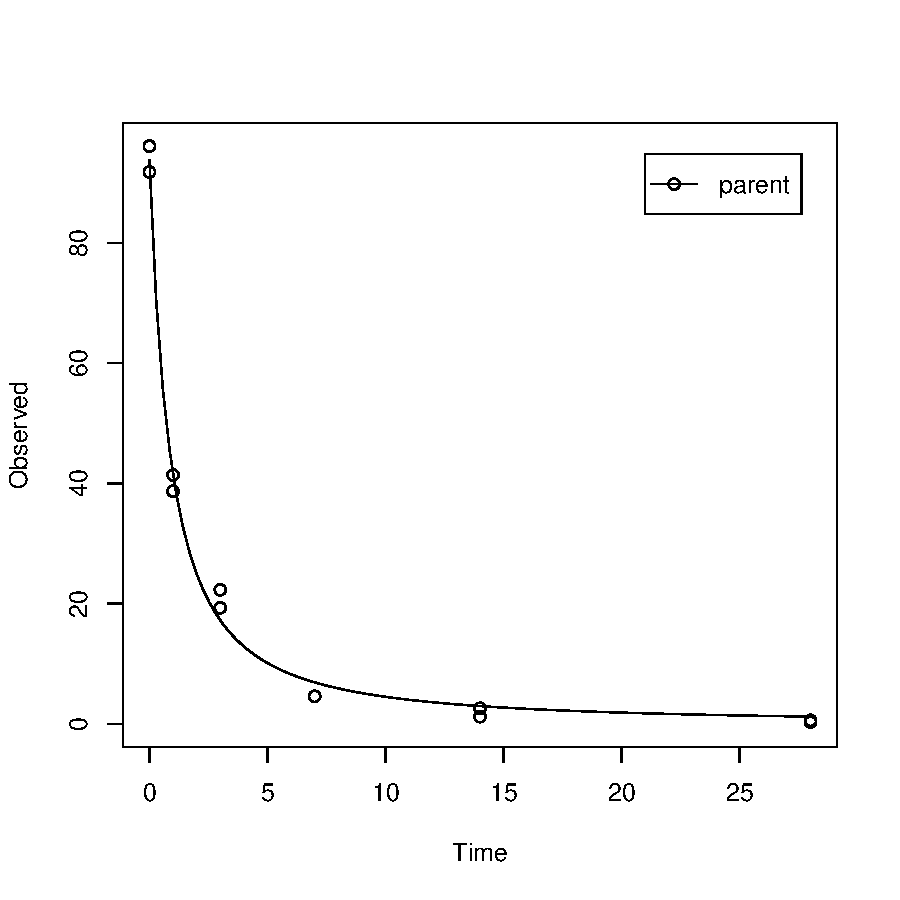
\includegraphics{examples-L2_FOMC}

The error level at which the $\chi^2$ test passes is much lower in this case.
Therefore, the FOMC model provides a better description of the data, as less
experimental error has to be assumed in order to explain the data.

Fitting the four parameter DFOP model does not further reduce the 
$\chi^2$ error level. 

\begin{Schunk}
\begin{Sinput}
R> m.L2.DFOP <- mkinfit(DFOP, FOCUS_2006_L2_mkin, quiet=TRUE)
R> plot(m.L2.DFOP)
\end{Sinput}
\end{Schunk}
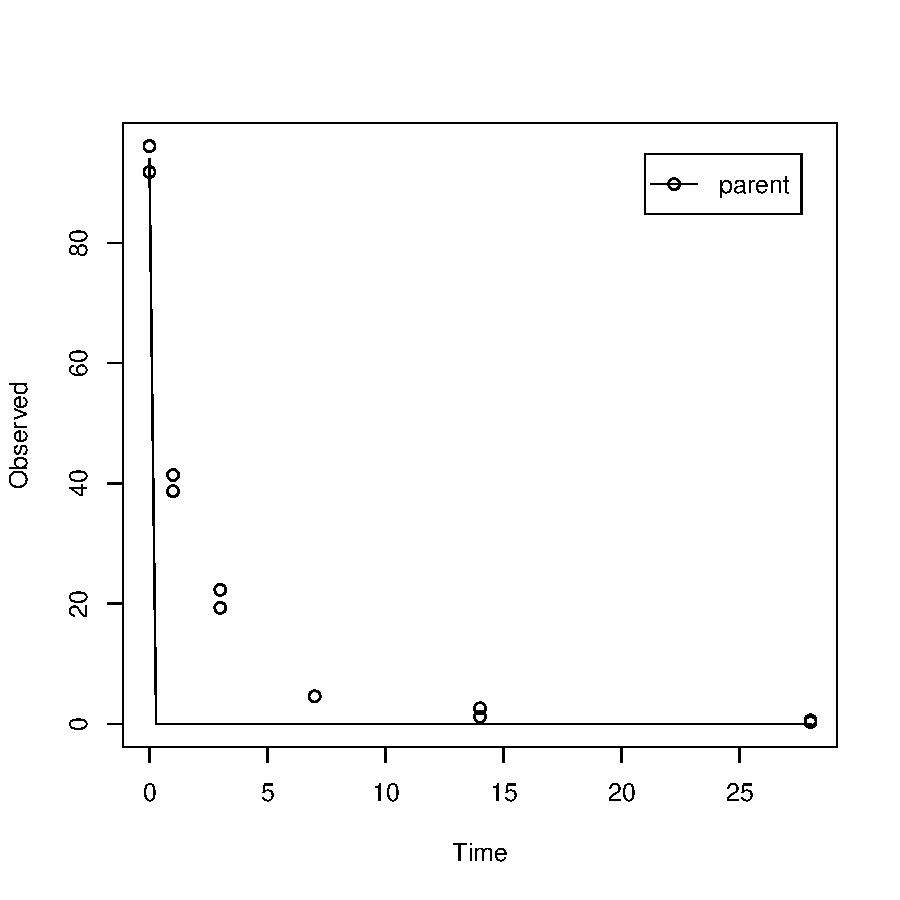
\includegraphics{examples-L2_DFOP}

Here, the default starting parameters for the DFOP model obviously do not lead
to a reasonable solution. Therefore the fit is repeated with different starting
parameters.

\begin{Schunk}
\begin{Sinput}
R> m.L2.DFOP <- mkinfit(DFOP, FOCUS_2006_L2_mkin, 
+   parms.ini = c(k1 = 1, k2 = 0.01, g = 0.8),
+   quiet=TRUE)
R> plot(m.L2.DFOP)
R> summary(m.L2.DFOP)
\end{Sinput}
\begin{Soutput}
mkin version:    0.9.10 
R version:       2.15.2 
Date of fit:     Sat Feb 16 21:38:16 2013 
Date of summary: Sat Feb 16 21:38:16 2013 

Equations:
[1] d_parent = - ((k1 * g * exp(-k1 * time) + k2 * (1 - g) * exp(-k2 * time)) / (g * exp(-k1 * time) + (1 - g) * exp(-k2 * time))) * parent

Starting values for optimised parameters:
         initial   type transformed
parent_0   1e+02  state 100.0000000
k1         1e+00 deparm   0.0000000
k2         1e-02 deparm  -4.6051702
g          8e-01 deparm   0.9802581

Fixed parameter values:
None

Optimised, transformed parameters:
         Estimate Std. Error
parent_0  93.9500         NA
k1         4.9589         NA
k2        -1.0880         NA
g         -0.2821         NA

Backtransformed parameters:
         Estimate
parent_0   93.950
k1        142.434
k2          0.337
g           0.402

Residual standard error: 1.732 on 8 degrees of freedom

Chi2 error levels in percent:
         err.min n.optim df
All data   2.529       4  2
parent     2.529       4  2

Estimated disappearance times:
       DT50 DT90
parent   NA   NA

Estimated formation fractions:
[1] ff
<0 rows> (or 0-length row.names)

Data:
 time variable observed predicted residual
    0   parent     96.1 93.950000   2.1500
    0   parent     91.8 93.950000  -2.1500
    1   parent     41.4 40.143423   1.2566
    1   parent     38.7 40.143423  -1.4434
    3   parent     19.3 20.464500  -1.1645
    3   parent     22.3 20.464500   1.8355
    7   parent      4.6  5.318322  -0.7183
    7   parent      4.6  5.318322  -0.7183
   14   parent      2.6  0.503070   2.0969
   14   parent      1.2  0.503070   0.6969
   28   parent      0.3  0.004501   0.2955
   28   parent      0.6  0.004501   0.5955
\end{Soutput}
\begin{Sinput}
R> s.m.L2.DFOP <- summary(m.L2.DFOP)
R> s.m.L2.DFOP$errmin
\end{Sinput}
\begin{Soutput}
            err.min n.optim df
All data 0.02528763       4  2
parent   0.02528763       4  2
\end{Soutput}
\end{Schunk}
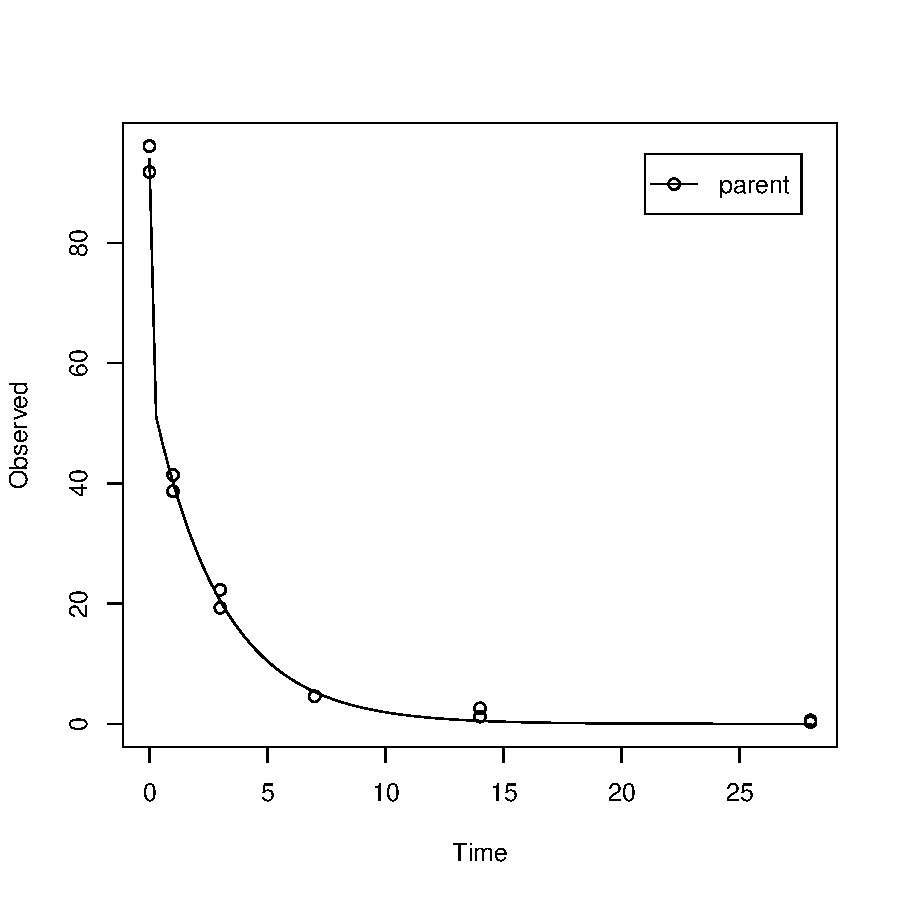
\includegraphics{examples-L2_DFOP_2}

Therefore, the FOMC model is clearly the best-fit model based on the 
$\chi^2$ error level criterion.

\subsection{Laboratory Data L3}

The following code defines example dataset L3 from the FOCUS kinetics
report, p. 290

\begin{Schunk}
\begin{Sinput}
R> library("mkin")
R> FOCUS_2006_L3 = data.frame(
+   t = c(0, 3, 7, 14, 30, 60, 91, 120),
+   parent = c(97.8, 60, 51, 43, 35, 22, 15, 12))
R> FOCUS_2006_L3_mkin <- mkin_wide_to_long(FOCUS_2006_L3)
\end{Sinput}
\end{Schunk}

SFO model, summary and plot:

\begin{Schunk}
\begin{Sinput}
R> m.L3.SFO <- mkinfit(SFO, FOCUS_2006_L3_mkin, quiet=TRUE)
R> summary(m.L3.SFO)
\end{Sinput}
\begin{Soutput}
mkin version:    0.9.10 
R version:       2.15.2 
Date of fit:     Sat Feb 16 21:38:16 2013 
Date of summary: Sat Feb 16 21:38:16 2013 

Equations:
[1] d_parent = - k_parent_sink * parent

Starting values for optimised parameters:
              initial   type transformed
parent_0        100.0  state  100.000000
k_parent_sink     0.1 deparm   -2.302585

Fixed parameter values:
None

Optimised, transformed parameters:
              Estimate Std. Error
parent_0        74.873      8.458
k_parent_sink   -3.678      0.326

Backtransformed parameters:
              Estimate
parent_0        74.873
k_parent_sink    0.025

Residual standard error: 12.91 on 6 degrees of freedom

Chi2 error levels in percent:
         err.min n.optim df
All data   21.24       2  6
parent     21.24       2  6

Estimated disappearance times:
        DT50  DT90
parent 27.43 91.12

Estimated formation fractions:
            ff
parent_sink  1

Parameter correlation:
              parent_0 k_parent_sink
parent_0        1.0000        0.5484
k_parent_sink   0.5484        1.0000

Data:
 time variable observed predicted  residual
    0   parent     97.8    74.873  22.92734
    3   parent     60.0    69.407  -9.40654
    7   parent     51.0    62.734 -11.73403
   14   parent     43.0    52.563  -9.56336
   30   parent     35.0    35.083  -0.08281
   60   parent     22.0    16.439   5.56137
   91   parent     15.0     7.510   7.48961
  120   parent     12.0     3.609   8.39083
\end{Soutput}
\begin{Sinput}
R> plot(m.L3.SFO)
\end{Sinput}
\end{Schunk}
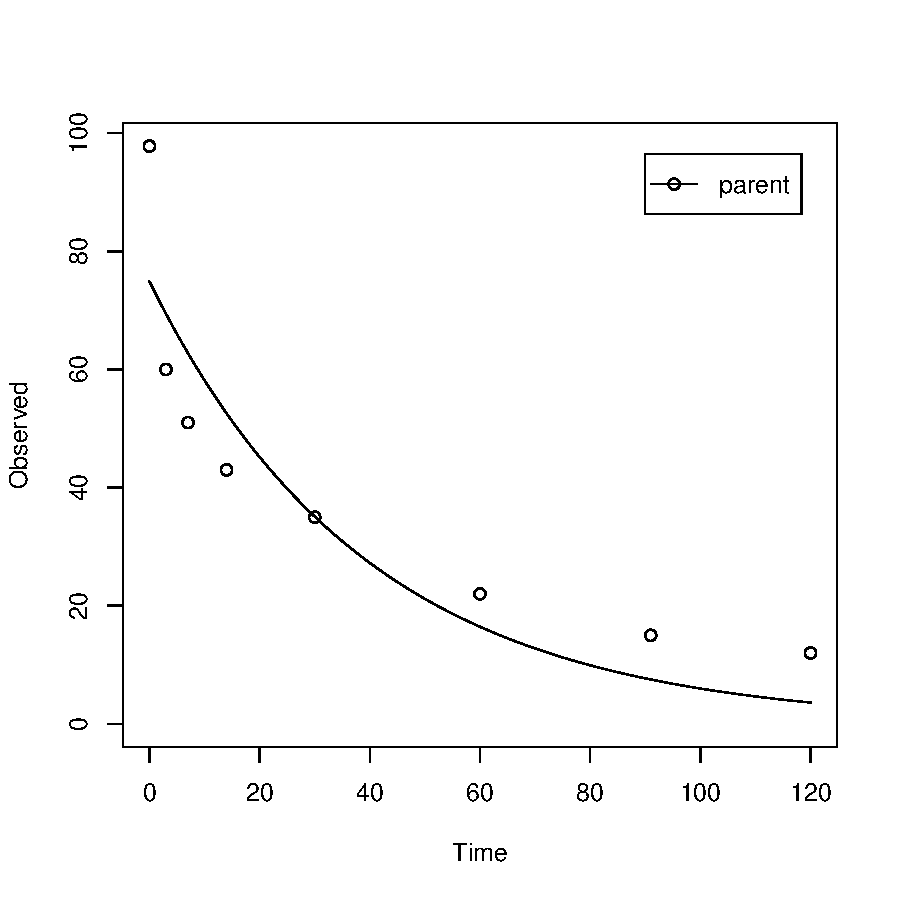
\includegraphics{examples-L3_SFO}

The $\chi^2$ error level of 22\% as well as the plot suggest that the model
does not fit very well. 

The FOMC model performs better:

\begin{Schunk}
\begin{Sinput}
R> m.L3.FOMC <- mkinfit(FOMC, FOCUS_2006_L3_mkin, quiet=TRUE)
R> plot(m.L3.FOMC)
R> s.m.L3.FOMC <- summary(m.L3.FOMC)
R> s.m.L3.FOMC$errmin
\end{Sinput}
\begin{Soutput}
            err.min n.optim df
All data 0.07321867       3  5
parent   0.07321867       3  5
\end{Soutput}
\begin{Sinput}
R> endpoints(m.L3.FOMC)
\end{Sinput}
\begin{Soutput}
$distimes
           DT50     DT90
parent 7.729478 431.2428

$ff
logical(0)

$SFORB
logical(0)
\end{Soutput}
\end{Schunk}
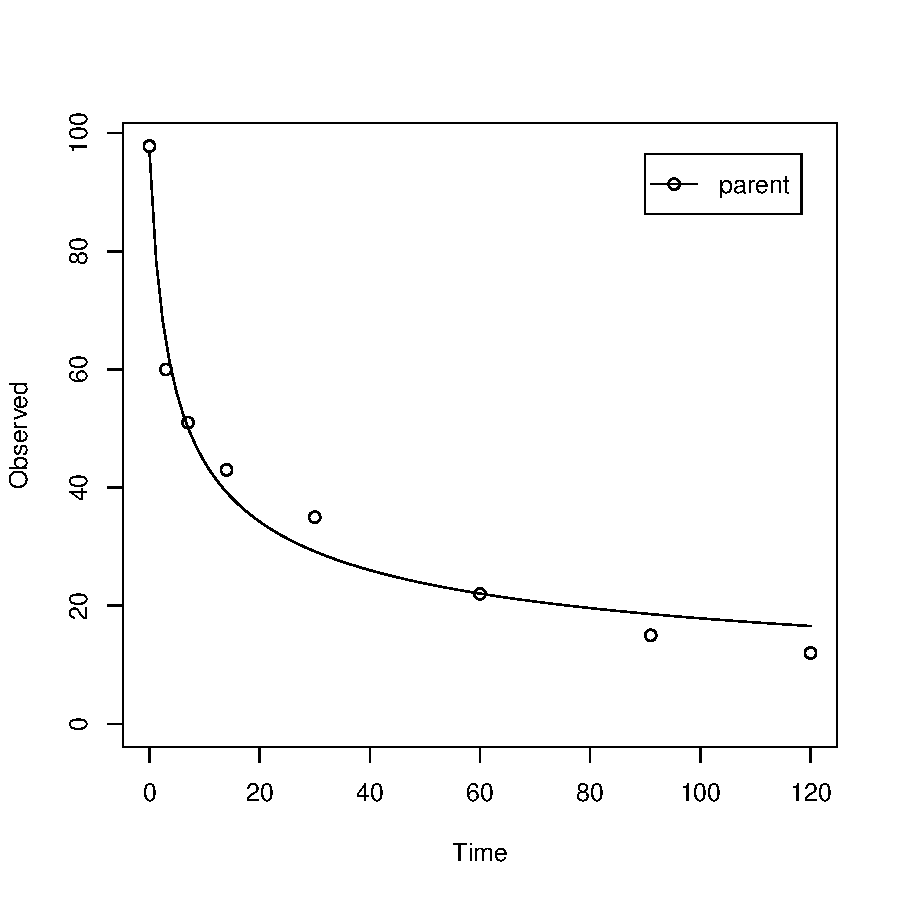
\includegraphics{examples-L3_FOMC}

The error level at which the $\chi^2$ test passes is 7\% in this case.

Fitting the four parameter DFOP model further reduces the $\chi^2$ error level
considerably:

\begin{Schunk}
\begin{Sinput}
R> m.L3.DFOP <- mkinfit(DFOP, FOCUS_2006_L3_mkin, quiet=TRUE)
R> plot(m.L3.DFOP)
R> s.m.L3.DFOP <- summary(m.L3.DFOP)
R> s.m.L3.DFOP$errmin
\end{Sinput}
\begin{Soutput}
            err.min n.optim df
All data 0.02223992       4  4
parent   0.02223992       4  4
\end{Soutput}
\end{Schunk}
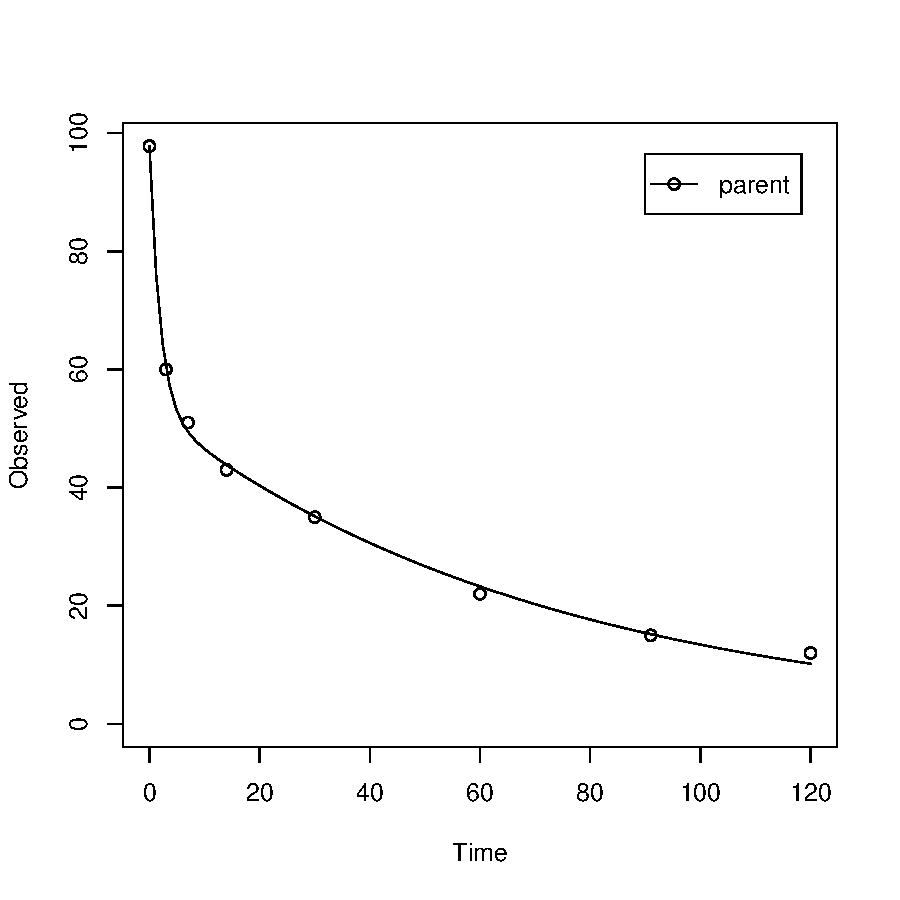
\includegraphics{examples-L3_DFOP}

Therefore, the DFOP model is the best-fit model based on the $\chi^2$ error
level criterion for laboratory data L3.

\subsection{Laboratory Data L4}

The following code defines example dataset L4 from the FOCUS kinetics
report, p. 293

\begin{Schunk}
\begin{Sinput}
R> library("mkin")
R> FOCUS_2006_L4 = data.frame(
+   t = c(0, 3, 7, 14, 30, 60, 91, 120),
+   parent = c(96.6, 96.3, 94.3, 88.8, 74.9, 59.9, 53.5, 49.0))
R> FOCUS_2006_L4_mkin <- mkin_wide_to_long(FOCUS_2006_L4)
\end{Sinput}
\end{Schunk}

SFO model, summary and plot:

\begin{Schunk}
\begin{Sinput}
R> m.L4.SFO <- mkinfit(SFO, FOCUS_2006_L4_mkin, quiet=TRUE)
R> summary(m.L4.SFO)
\end{Sinput}
\begin{Soutput}
mkin version:    0.9.10 
R version:       2.15.2 
Date of fit:     Sat Feb 16 21:38:17 2013 
Date of summary: Sat Feb 16 21:38:17 2013 

Equations:
[1] d_parent = - k_parent_sink * parent

Starting values for optimised parameters:
              initial   type transformed
parent_0        100.0  state  100.000000
k_parent_sink     0.1 deparm   -2.302585

Fixed parameter values:
None

Optimised, transformed parameters:
              Estimate Std. Error
parent_0         96.44      1.949
k_parent_sink    -5.03      0.080

Backtransformed parameters:
              Estimate
parent_0        96.442
k_parent_sink    0.007

Residual standard error: 3.651 on 6 degrees of freedom

Chi2 error levels in percent:
         err.min n.optim df
All data   3.288       2  6
parent     3.288       2  6

Estimated disappearance times:
       DT50 DT90
parent  106  352

Estimated formation fractions:
            ff
parent_sink  1

Parameter correlation:
              parent_0 k_parent_sink
parent_0        1.0000        0.5865
k_parent_sink   0.5865        1.0000

Data:
 time variable observed predicted residual
    0   parent     96.6     96.44   0.1585
    3   parent     96.3     94.57   1.7324
    7   parent     94.3     92.13   2.1744
   14   parent     88.8     88.00   0.7972
   30   parent     74.9     79.26  -4.3589
   60   parent     59.9     65.14  -5.2376
   91   parent     53.5     53.18   0.3167
  120   parent     49.0     43.99   5.0054
\end{Soutput}
\begin{Sinput}
R> plot(m.L4.SFO)
\end{Sinput}
\end{Schunk}
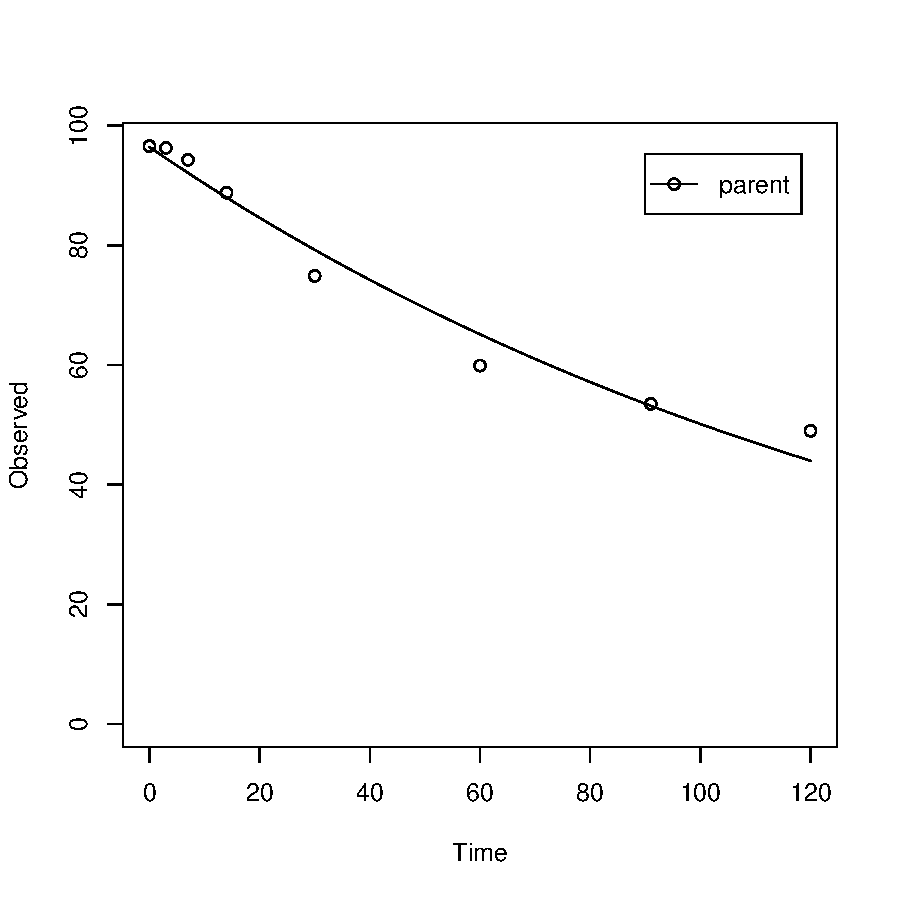
\includegraphics{examples-L4_SFO}

The $\chi^2$ error level of 3.3\% as well as the plot suggest that the model
fits very well. 

The FOMC model for comparison

\begin{Schunk}
\begin{Sinput}
R> m.L4.FOMC <- mkinfit(FOMC, FOCUS_2006_L4_mkin, quiet=TRUE)
R> plot(m.L4.FOMC)
R> s.m.L4.FOMC <- summary(m.L4.FOMC)
R> s.m.L4.FOMC$errmin
\end{Sinput}
\begin{Soutput}
            err.min n.optim df
All data 0.02027643       3  5
parent   0.02027643       3  5
\end{Soutput}
\end{Schunk}
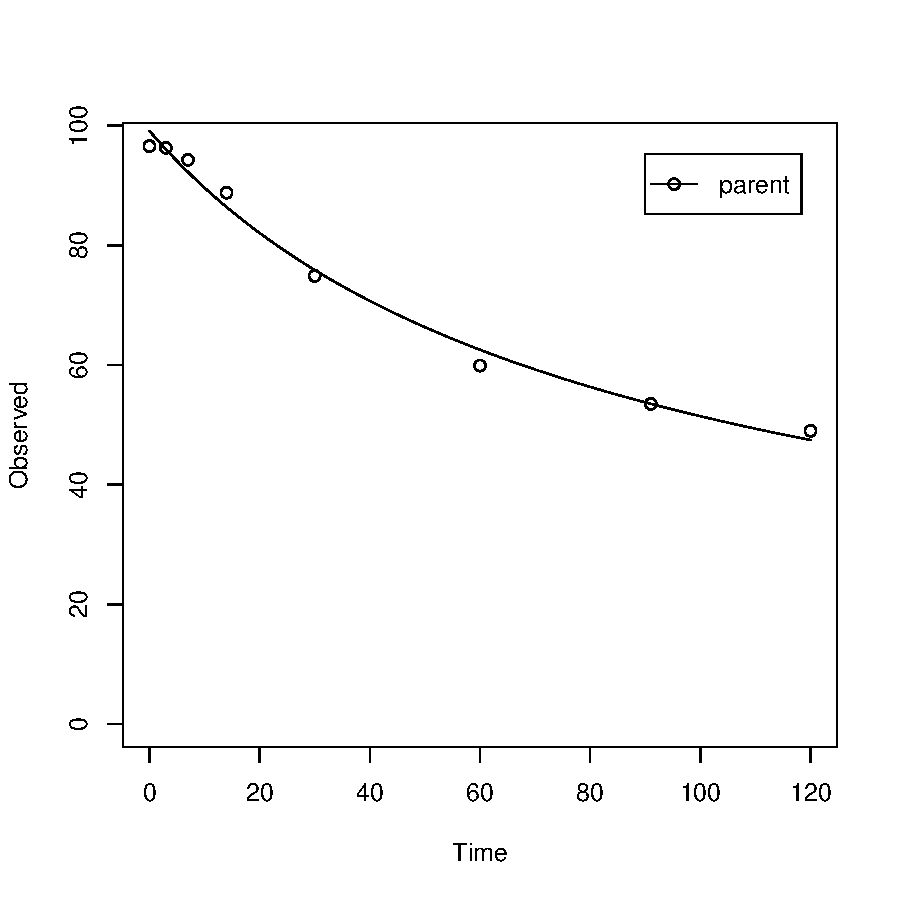
\includegraphics{examples-L4_FOMC}

The error level at which the $\chi^2$ test passes is slightly lower for the FOMC 
model. However, the difference appears negligible.

\bibliographystyle{plainnat}
\bibliography{references}

\end{document}
% vim: set foldmethod=syntax:
